\documentclass[12pt]{article}

\usepackage[top=1in, bottom=1in, left=1in, right=1in]{geometry}
\usepackage{fancyhdr}
\usepackage{graphicx}

\pagestyle{fancy}
\lhead{}
\chead{Finding the optimal configuration for a renewable power plant using a genetic algorithm}
\rhead{}
\lfoot{}
\cfoot{\thepage}
\rfoot{}

\begin{document}

\title{Finding the optimal configuration for a renewable power plant using a genetic algorithm}
\author{Donnelly Baart, Luc Bontan, Jeremy van Dijk, Michiel Maas, Aurin Spaninks}
\date{\today}
\maketitle

\section*{Abstract}

Write the summary here

\section*{Keywords}

Genetic algorithm, Renewable energy


\newpage

\section{Introduction}
Electricity is increasingly being generated by wind turbines and solar panels. The disadvantage is that production varies due to weather influences. As a result, electricity supply and demand do not match each other. This makes it difficult for these to compete with traditional power plants using fossil fuels.

The research group Energy in Transition at The Hague University of Applied Sciences asked us for a way to find the cheapest configuration of solar panels, wind turbines and energy storage to deliver a constant supply of electricity. This could then be used to get the optimal configuration for various geographic regions and different levels of demand.

The research group provided a simulation to calculate the hourly electricity production for a whole year using a particular configuration of wind turbines and solar panels. We decided to use a genetic algorithm in conjunction with this simulation to approximate the optimal renewable energy setup.

\section{Simulation}

\section{Cost calculation}

\subsection{Parts}

\subsection{Storage}

We need to calculate the minimum amount of required storage to calculate the total cost. If this calculation is not fast enough it will slow down training considerably. The following is a rough explanation of the method used. The simulation returns an array of 8760 hours. In figure \ref{fig:storage} we use an array of 52 weeks with fake values for simplicity.

\begin{figure}[h!]
\center{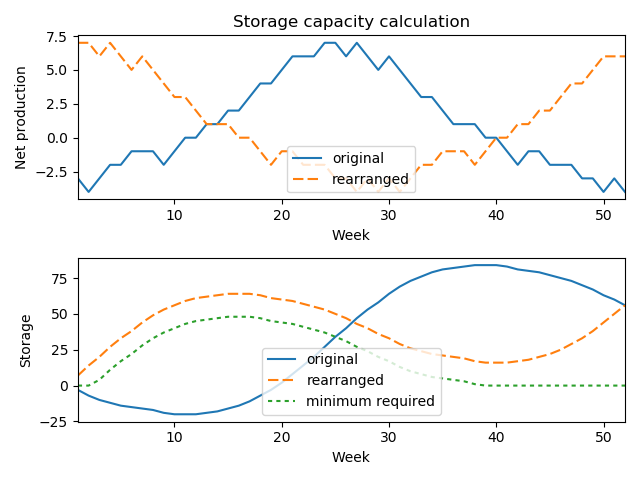
\includegraphics[width=10cm]{storage_plot.png}}
\caption{\label{fig:storage} Steps for calculating the minimum required storage cost}
\end{figure}

We take the array and subtract the required energy to get the net production. We then make a cumulative array to show the total storage at any given point. If the last value in this array is positive, we do not have a deficit. We then rearrange the original net production in such a way that the storage array never dips below zero by choosing a different starting point. In figure \ref{fig:storage} we chose to start in week 24. We again make a cumulative array for the storage. Finally, the rearranged storage array is lowered wherever possible. The minimum required amount storage is the highest value in this array.

\section{Genetic algorithm}

We used a mostly standard genetic algorithm. We used populations of 100 and selected some of the best to generate the next generation. However, we also calculated which configurations were the most different from the rest and selected some of those as well as some random ones. These last two measures are there to prevent local minimums. We also added some random mutations.

\section{Findings}

\section{Conclusion}

\section{Acknowledgments}

This is a fake citation \cite{FakeArticle}

\newpage

\bibliography{RenewablePowerPlant} 
\bibliographystyle{ieeetr}

\end{document}